\normaltrue \difficilefalse \tdifficilefalse
\correctionfalse
%\UPSTIidClasse{11} % 11 sup, 12 spé
%\newcommand{\UPSTIidClasse}{11}

\exer{Scooter Piaggio$\star$ \label{B2:16:81}}
%% 
\setcounter{numques}{0}
\UPSTIcompetence[2]{B2-16}
\index{Compétence B2-16}

\index{Scooter Piaggio}
\index{Hyperstatisme}

\ifcorrection
\else
\textbf{Pas de corrigé pour cet exercice.}
\fi


\ifprof
\else
On s'intéresse au système direction du scooter Piaggio.

\begin{figure}[H]
\centering
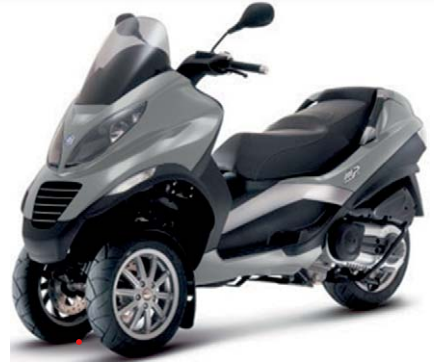
\includegraphics[width=.45\linewidth]{81_01.png}
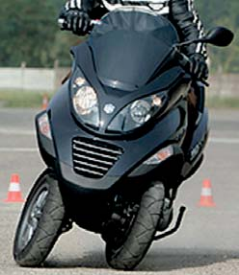
\includegraphics[width=.45\linewidth]{81_02.png}
%\caption{Pince utilisée sur le système ROBOVOLC et schéma cinématique associé \label{fig_23}}
\end{figure} 



\begin{figure}[H]
\centering
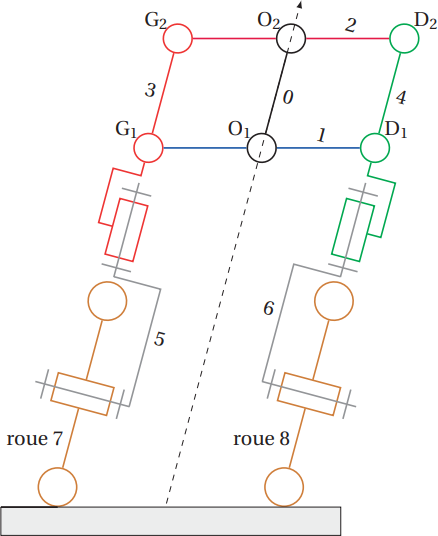
\includegraphics[width=\linewidth]{81_03.png}
%\caption{Pince utilisée sur le système ROBOVOLC et schéma cinématique associé \label{fig_23}}
\end{figure} 
\fi

\question{Réaliser le graphe de liaisons du système de direction. On considèrera le sol comme une classe d'équivalence.}

\question{Calculer le degré d'hyperstatisme.}

\question{Si le modèle est hyperstatique, modifier le modèle pour le rendre isostatique.}
 

\ifprof
\else

%\noindent\footnotesize
% \fbox{\parbox{.9\linewidth}{
% Éléments de corrigé : 
% \begin{enumerate}
%\item .
%%\item $h=8$.
%\item .
% \end{enumerate}}}
%\normalsize

\begin{flushright}
\footnotesize{Corrigé  voir \ref{B2:16:81}.}
\end{flushright}%
\fi